\vspace{1cm}
\fancyhead[C]{\normalsize\textbf{$\qquad$ Teil I: Offene Aufgaben}}
\renewcommand{\labelenumi}{\theenumi.}
\section*{Aufgabe 1 (38 Punkte)}
\vspace{0.4cm}
%\titleformat{\subsection}[runin]
%{\normalfont\large\bfseries}{\thesubsection}{1em}{}
\subsection*{\aufgabe{a1}{8}} 
Die Wirtschaftsredakteurin eines wichtigen Verlagshauses zieht in Betracht,
kostenlose Exemplare eines Buchs an Dozierende der Wirtschaftswissenschaften an Schweizer Hochschulen zu verschicken, da sie weiss, dass Dozierende dazu neigen, Bücher als Kurslektüre auszuwählen, die sie bereits in ihren Regalen stehen haben. Die Fixkosten dieser Werbekampagne belaufen sich auf $100'000$ Schweizer Franken.
Die Stückkosten eines einzelnen Buchs betragen $10$ Schweizer Franken, im Handel werden die Bücher schließlich für $40$ Schweizer Franken pro Exemplar verkauft.
Auf der Basis historischer Daten schätzt die Redakteurin, dass wenn $x$ Gratisexemplare versendet werden, ein Verkauf von insgesamt
\begin{align*}
	B(x) = 20'000 - 19'000 e^{-0.0002 x }
\end{align*}
Exemplaren des Buchs erzielt wird. \\
\\
Zeigen Sie, dass wenn die Produktion auf maximal $6'000$ Bücher beschränkt ist, es genau eine Menge $ x^\star \in (0, 6'000)$ an Gratisexemplaren gibt, bei der die Gesamtkosten genau durch den Umsatz gedeckt werden.
\
\\ \\
\textbf{Lösung:}
\begin{mdframed}
\underline{\textbf{Vorgehensweise:}}
\renewcommand{\labelenumi}{\theenumi.}
\begin{enumerate}
\item 
Stelle den mathematischen Rahmen her.
\item
Überlege wie man die Existenz und Eindeutigkeit zeigt.
\item
Wende den Nullstellensatz von Bolzano an und zeige die Eindeutigkeit. 

\end{enumerate}
\end{mdframed}
\underline{1. Stelle den mathematischen Rahmen her}\\
Zunächst werden wir den mathematischen Rahmen herstellen. Damit wissen wir welches Problem angegangen wird und wir können die passenden Konzepte anwenden.\\
\\
In dieser Aufgabe suchen wir nach der Existenz und Eindeutigkeit einer Anzahl $x^\star $ an kostenlosen Exemplaren, ab welcher alle Kosten gedeckt sind und die Redakteurin beginnt Gewinne zu machen. Den Gewinn abhängig von den kostenlosen Exemplaren $x$ können wir formalisiert durch
\begin{align*}
	G(x) = \underbrace{40 \ B(x)}_{\textrm{Verkaufserlöse}} - \underbrace{(10 B(x) - 10 x)}_{\textrm{Produktionskosten}} - \underbrace{100000}_{\textrm{Fixkosten}}, \quad
	x \in (0, 6000).
\end{align*}
beschreiben. Wir suchen nun nach der Anzahl kostenloser Exemplare $x^\star$, sodass 
\begin{align*}
G(x^\star ) = 0
\end{align*}
mit $G(x) < 0$ für $0 \leq x < x^\star$ und $G(x) > 0$ für $x^\star < x \leq 6000$ gilt.\\
\\

\underline{2. Überlege wie man die Existenz und Eindeutigkeit zeigt}\\
Um zu zeigen, dass ein $x^\star  \in (0,6000)$ mit
\begin{align*}
	G(x^\star)= 0
\end{align*}
existiert, können wir den Nullstellensatz von Bolzano anwenden. Dieser besagt:\\
Sei $G:[a,b] -> \R$ eine stetige Funktion mit $G(a) < 0 \wedge G(b) > 0 $ oder $G(a) > 0 \wedge G(b) < 0$\\
Dann existiert mindestens ein $x^\star \in [a,b]$, sodass $G(x^\star) = 0$ gilt.\\
\\
In unserem Fall ist $a = 0 $ und $b = 6000$.
Damit wissen wir jedoch nur, dass eine Nullstelle existiert. Es könnten auch mehrere Nullstellen in $[0,6000]$ existieren. 
Falls $G $ auf $[0,6000]$ streng monoton ist, kann jeder Wert auf diesem Intervall nur einmal getroffen werden und wir erreichen die Eindeutigkeit.\\
\\
\underline{3. Wende den Nullstellensatz von Bolzano an und zeige die Eindeutigkeit}\\
Für die Gewinnfunktion gilt:
\begin{align*}
	G(x)
	&= 
	40 B(x) 
	- ( B(x) + 10 x) - 100000
	= 
	40 B(x) 
	-  B(x) -10 x - 100000\\
	&=
	30 B(x) - 10 x - 100000\\
	&=
	30 
	\left(
	20'000 - 19'000 e^{-0.0002 x }
	\right)
	- 10x - 100000\\
	&=
	600000 - 570000 e^{-0.0002 x } - 10 x - 100000\\
	&= 
	500000 - 570000 e^{-0.0002 x } - 10 x.
\end{align*}
Als Zusammensetzung stetiger Funktionen ist $G$ stetig. Damit können wir versuchen den Nullstellensatz anzuwenden. An den Rändern des relevanten Intervalls gilt:
\begin{align*}
	G(0) 
	&= 500000 - 570000 \cdot e^{-0.0002 \cdot 0 } - 10 \cdot  0
	= 500000 - 570000  = - 70000 < 0 \\
	G(60000)
	&=
	500000 - 570000 \cdot e^{-0.0002 \cdot 6000 } - 10 \cdot 6000
	=
	500000 - 570000 \cdot e^{-\frac{2}{10000} \cdot 6000 } - 60000\\
	&=
	440000 - 570000 \cdot e^{-\frac{12000}{10000}  } 
	=
	440000 - 570000 \cdot e^{-\frac{12}{10}  } 
	>
	440000 - 570000 \cdot e^{-\frac{10}{10}  } \\
	&=
	440000 - 570000 \cdot \frac{1}{e}
	>
	440000 - 570000 \cdot \frac{1}{2}\\
	&= 440000 - 285000 = 155000 > 0.
\end{align*}
Für die rechte Seite des Intervalls ist es empfehlenswert den Taschenrechner zu verwenden. Dies soll $e \approx 2.71....$ zeigen, wie es auch ohne geht. 
Wegen $G(0) < 0$ und $G(6000) > 0$ existiert nach dem Nullstellensatz von Bolzano in dem Intervall $(0,6000)$ mindestens eine Nullstelle. Für die Eindeutigkeit betrachten wir die Ableitung:
\begin{align*}
	G^\prime(x)
	&=
	-570000 ( - 0.0002) e^{-0.0002 x} - 10
	=
	57 \cdot 2 e^{-0.0002 x} - 10
	=
	114 \cdot e^{-0.0002 x}- 10\\
	&> 
	114 \cdot e^{-0.0002 \cdot 6000} - 10
	=
	114 \cdot e^{-\frac{12}{10}} - 10 \approx 24.34  > 0, 
	\quad x \in ( 0 , 6000).
\end{align*}
Damit ist $G$ auf dem Intervall streng monoton wachsend und es existiert ein eindeutiges $x^\star \in (0,6000) $, sodass 
\begin{align*}
	G(x^\star) = 0
\end{align*} 
mit $G(x) < 0$ für $0 \leq x < x^\star$ und $G(x) > 0$ für $x^\star < x \leq 6000$ gilt.
\newpage

\subsection*{\aufgabe{a2}{8}}
Die Wirtschaftsredakteurin eines wichtigen Verlagshauses zieht in Betracht,
kostenlose Exemplare eines Buchs an Dozierende der Wirtschaftswissenschaften an Schweizer Hochschulen zu verschicken, da sie weiss, dass Dozierende dazu neigen, Bücher als Kurslektüre auszuwählen, die sie bereits in ihren Regalen stehen haben. Die Fixkosten dieser Werbekampagne belaufen sich auf $100'000$ Schweizer Franken.
Die Stückkosten eines einzelnen Buchs betragen $10$ Schweizer Franken, im Handel werden die Bücher schließlich für $40$ Schweizer Franken pro Exemplar verkauft.
Auf der Basis historischer Daten schätzt die Redakteurin, dass wenn $x$ Gratisexemplare versendet werden, ein Verkauf von insgesamt
\begin{align*}
	B(x) = 20'000 - 19'000 e^{-0.0002 x }
\end{align*}
Exemplaren des Buchs erzielt wird. Wenn die Produktion auf maximal $6'000$ Bücher beschränkt ist, gibt es genau eine Menge $ x^\star \in (0, 6'000)$ an Gratisexemplaren, bei der die Gesamtkosten genau durch den Umsatz gedeckt werden.\\
\\
Verwenden Sie eine Taylor-Approximation zweiter Ordnung im Punkt $x_0 = 750$, um eine Näherung für $x^\star$ zu finden.
\\
 \\
\textbf{Lösung:}
\begin{mdframed}
\underline{\textbf{Vorgehensweise:}}
\renewcommand{\labelenumi}{\theenumi.}
\begin{enumerate}
\item Bestimme das Taylorpolynom.
\item Bestimme die Näherungslösung. 
\end{enumerate}
\end{mdframed}

\underline{1. Bestimme das Taylorpolynom}\\
In dieser Aufgabe ist eine Näherungslösung für die Anzahl der Exemplare $x^\star$ ab welcher die Kosten gedeckt sind gesucht. Wir suchen also eine Näherungslösung für die Gleichung
\begin{align*}
	G(x) = 0
\end{align*}
Wir verwenden nun das Taylorpolynom zweiter Ordnung $P_2$ von $G$ in dem Entwicklungspunkt $x_0 = 750$ um die Gleichung
\begin{align*}
	P_2(x) = 0
\end{align*}
als Approximation der Gleichung $G(x) = 0$ zu lösen. Das Taylorpolynom $P_2$ ist gegeben durch:
\begin{align*}
	P_2(x)
	=
	G(750) 
	+ G^\prime(750) (x - 750)
	+ \frac{G^{\prime \prime}(750)}{2} (x - 750)^2.
\end{align*}
Mit der Teilaufgabe (a1)  erhalten wir:
\begin{align*}
	a_0 &:= G(750) 
	= 
	500000 - 570000 e^{-0.0002 \cdot 750 } - 10 \cdot 750
	\approx  1896.4534\\
	a_1 &:= G^\prime(750)
	=
	114 \cdot e^{-0.0002 \cdot  750}- 10
	\approx 88.1207
\end{align*}
Für den letzten Koeffizienten $a_2 := G^{\prime \prime}(750)$ müssen wir die zweite Ableitung berechnen:
\begin{align*}
	G^{\prime \prime}(x)
	=
	\frac{\mathrm{d}}{\mathrm{dx}}
	\left(
			114 \cdot e^{-0.0002 x}- 10
	\right)
	=
	114 \cdot  ( -0.0002) \cdot e^{-0.0002 x}
	=
	-0.0228 \cdot e^{-0.0002 x}.
\end{align*}
Damit erhalten wir
\begin{align*}
	a_2 : = G^{\prime \prime}(750)
	= -0.0228 \cdot e^{-0.0002 \cdot 750}
	\approx
	-0.0196.	
\end{align*}
Das Taylorpolynom $P_2$ ist somit durch 
\begin{align*}
	P_2(x)
	= 
	a_0 
	+ 
	a_1(x - 750)
	\frac{1}{2}
	a_2 
	(x - 750)^2 	
	\approx
	1896.4534
	+
	88.1207
	(x - 750)
	+
	\frac{1}{2}
	(-0.0196) (x - 750)^2
\end{align*}
gegeben.\\
\\
\underline{2. Bestimme die Näherungslösung}\\
Wir substituieren $s = x - 750$, wodurch uns das Lösen der Gleichung
\begin{align*}
	P_2(x) = a_0 
	+ 
	a_1(x - 750)
	+
	\frac{1}{2}
	a_2 
	(x - 750)^2 	
	=
	a_0 + a_1 s +\frac{1}{2} a_2 s^2 = 0
\end{align*}
erleichtert wird. Mit der $abc$- Formel erhalten wir:
\begin{align*}
	s_{1,2}
	&=
	\frac{-a_1 \pm \sqrt{a_1^2 - 4 \frac{1}{2} a_2 a_0}}{2 \frac{1}{2} a_2}
	=
	\frac{-a_1 \pm \sqrt{a_1^2 - 2  a_2 a_0}}{ a_2} \\
	&\approx
	\frac{-88.1207 \pm \sqrt{88.1207^2 + 2 \cdot 0.0196 \cdot 1896.4534}}{-0.0196}\\
	&=
	\frac{88.1207 \pm \sqrt{88.1207^2 + 2 \cdot 0.0196 \cdot 1896.4534}}{0.0196}
	\in 
	\{ -21.47, 9013.378\}.
\end{align*}
Mit der Rücksubstitution $x = s + 750$ erhalten wir die Lösungen 
\begin{align*}
	x
	\in 
	\{
	728.530,9763.378
	\}.
\end{align*}
Die zweite Lösung liegt nicht in dem Intervall $(0,6000)$. Die relevante Lösung ist $x = 728.530$. Damit gilt $x^\star \approx 728.530$.


\newpage
\subsection*{\aufgabe{b}{12}}
Anne und Robert haben gerade erfolgreich ihr Masterprogramm in Quantitativen
Methoden an der Universität St.Gallen abgeschlossen und sind nun dabei, ihre eigene
Firma AlgoTrade aufzubauen, die Machine Learning Algorithmen für den computergesteuerten Handel an Finanzmärkten entwickelt. Sie haben bereits viele vielversprechende Ideen, jedoch fehlt ihnen das Eigenkapital. Die anfänglichen Investitionen für den Kauf der IT-Infrastruktur und für die Entwicklung der Software belaufen sich auf $1'500'000$ Schweizer Franken.
Ein Risikokapitalgeber ist zu einem Investment in Höhe von $500'000$ Schweizer Franken bereit, verlangt aber im Gegenzug einen Anteil von $30 \%$ an der Firma.
Zusätzlich nehmen Anne und Robert am 1. Januar 2022 einen Kredit in Höhe von $1'000'000$ Schweizer Franken zu einem jährlichen Zinssatz von $2 \% $ auf.
Die Bank verlangt dabei, dass $40 \%$ des geschuldeten Betrags bis Ende 2026 über konstante Zahlungen $C$, fällig jeweils am Jahresende, zurückgezahlt sein muss.
\begin{enumerate}
	\item[(b1)] Fügen Sie die Ereignisse und Mittelflüsse dem Zeitstrahl hinzu.
	\item[(b2)] Berechnen Sie die Höhe der Ratenzahlung $C$.
\end{enumerate}
Bereits nach 3 Jahren ist AlgoTrade sehr erfolgreich und generiert beträchtliche Umsätze. Beginnend mit der nächsten Rückzahlung am 31. Dezember 2025 wollen Anne und Robert jeweils $180'000$ Schweizer Franken am Ende jedes Jahres solange zurückzahlen, bis die bestehende Restschuld komplett getilgt ist.
\begin{enumerate}
	\item[(b3)] Ergänzen Sie die Information am Zeitstrahl und berechnen Sie die Restschuld am 1. Januar 2025, also direkt nach der jüngsten Rückzahlung.
	\item[(b4)] Am 1. Januar 2029, direkt nach der jüngsten Rückzahlung, verkaufen Anne und Robert	ihre Firma für $5'000'000$ Schweizer Franken und tilgen mit ihrem Anteil die bestehende	Restschuld. Wie hoch ist ihr Gewinn?
\end{enumerate}
\begin{center}
	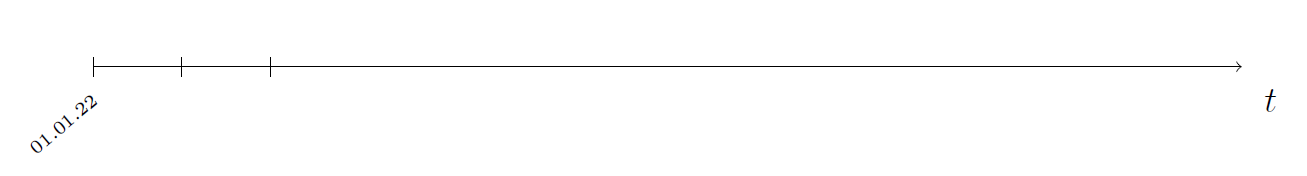
\includegraphics[scale=0.45]{pictures/zeitstrahl_1_b}
\end{center}
\newpage
\textbf{Lösung:}
\begin{mdframed}
\underline{\textbf{Vorgehensweise:}}
\begin{enumerate}
\item[(b1)] 
Füge die Ereignisse und Mittelflüsse zum Zeitstrahl hinzu.
\item[(b2)]
\begin{enumerate}
	\item[1.] Für die Ratenzahlung $C$ gibt es mehrere Interpretationen. Zähle diese auf.
	\item[2.] 
	Berechne die verschiedenen Interpretationen.
\end{enumerate}
\item[(b3)]
\begin{enumerate}
	\item[1.] Ergänze die Information am Zahlenstrahl.
	\item[2.] 
	Berechne die Restschuld.
\end{enumerate}
\end{enumerate}
\end{mdframed}

\underline{(b1) Füge die Ereignisse und Mittelflüsse zum Zeitstrahl hinzu}\\
\begin{center}
	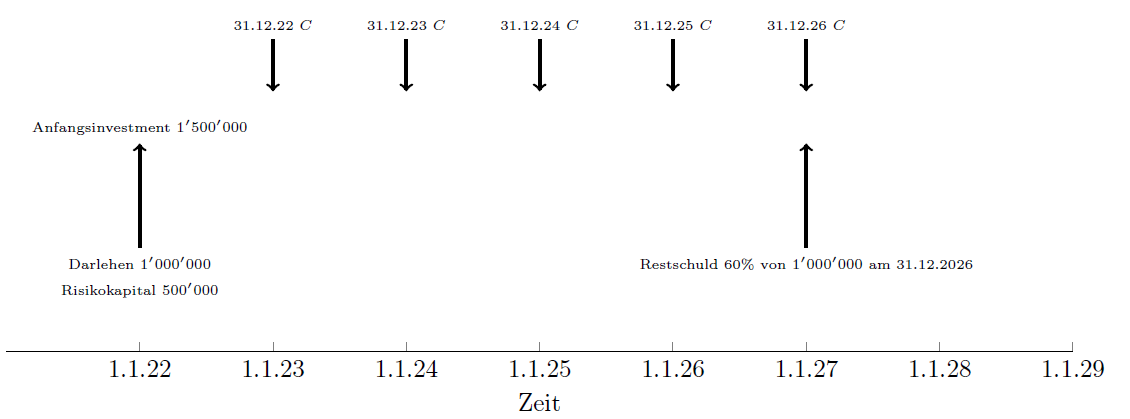
\includegraphics[scale=0.6]{pictures/zeitstrahl_1_b_filled_1}
\end{center}

\underline{(b2) 1. Für die Ratenzahlung $C$ gibt es mehrere Interpretationen. Zähle diese auf}\\
Wie wir die Lösung der Aufgabe angehen hängt von der Interpretation der Information, dass $40 \%$ des geschuldeten Betrags bis Ende 2026 zurückgezahlt werden muss, ab.
\begin{enumerate}
	\item 
	Die Zahlungen $C$ werden so gewählt, dass die Restschuld Ende 2026 noch $60 \%$ des Kreditbetrags, also $600000$ Schweizer Franken, beträgt.
	In der Praxis ist dies die gängige Interpretation.
	\item 
	Die Zahlungen $C$ werden so gewählt, dass ihr Wert 2026 $40 \%$ des Kreditbetrags, also $400000$ Schweizer Franken, beträgt.
	\item 
	DIe Zahlungen $C$ werden so gewählt, dass ihr Wert Anfang 2022 $40 \%$ des Kreditbetrags, also $400000$ Schweizer Franken, beträgt.
	Dies ist äquivalent dazu, dass dieser Wert Ende 2026 $40 \%$ der über fünf Jahre aufgezinsten Kreditsumme, d.h. $40 \% \cdot 1000000 \cdot ( 1 + 2 \%)^5$, entspricht. 
\end{enumerate}

\underline{(b2) 2. Berechne die verschiedenen Interpretationen}\\
\\
\textbf{Interpretation 1:}
Zunächst berechnen wir die bestehende Restschuld am 31.12.2026, wenn keine Zahlungen $C$ erfolgen:
\begin{align*}
	RS_{\mathrm{31.12.2026}}
	=
	RS_{\mathrm{1.1.2022}} ( 1+ 2 \%)^5
	=
	1 000 000 \cdot 1.02^5 
	\approx
	1 104 080.80 \ \textrm{(Schweizer Franken)}.
\end{align*}
Diese werden wir benötigen um die Zahlungen $C$ zu bestimmen.
Die bestehende Restschuld sollte zum 31.12.2026 $60 \%$ der $1 000 000$ Schweizer Franken betragen.
Damit erhalten wir für Ende 2026 folgenden kumulierten Wert der konstanten Zahlungen $C$, welche jeweils über fünf Jahre zum Jahresende bezahlt werden, durch
\begin{align*}
	RS_{\mathrm{31.12.2026}}
	- 600 000 
	\approx 
	504 080.85
	\ \textrm{(Schweizer Franken)}.
\end{align*} 
Somit kennen wir den Endwert der fünfjährigen nachschüssigen Rente $C$. Hiermit können wir mit der Endwertformel die Zahlungen $C$ berechnen:
\begin{align*}
	&C \frac{(1+2\%)^5 -1 }{2 \%} = 	RS_{\mathrm{31.12.2026}}
	- 600 000\\
	\ \Leftrightarrow \
	&C_1:=C 
	= (RS_{\mathrm{31.12.2026}}
	- 600 000) \cdot \frac{2 \%}{1+2\%)^5 -1 }
	=
	\frac{504 080.85 \cdot 2 \%}{1+2\%)^5 -1 }
	\approx 96 863.35
	\ \textrm{(Schweizer Franken)}.
\end{align*}
\ \\
\textbf{Interpretation 2:}
Bei den konstanten Zahlungen $C$ handelt es sich um eine nachschüssige Rente, welche über fünf Jahre gezahlt wird.
Mit der zweiten Interpretation erhalten wir durch die Endwertformel:
\begin{align*}
	400 000
	=
	C \frac{(1+2\%)^5 -1 }{2 \%}
	\ \Leftrightarrow \
	C_2 := C
	&= 400 000 \cdot
	\frac{2 \%}{(1+2\%)^5 -1}
	=
	\frac{ 400 000 \cdot 2 \%}{(1+2\%)^5 -1}\\
	&\approx
	76 863.35
	\ \textrm{(Schweizer Franken)}.
\end{align*}
\ \\
\textbf{Interpretation 3:}
Zunächst berechnen wir die bestehende Restschuld am 31.12.2026, wenn keine Zahlungen $C$ erfolgen:
\begin{align*}
	RS_{\mathrm{31.12.2026}}
	=
	RS_{\mathrm{1.1.2022}} ( 1+ 2 \%)^5
	=
	1 000 000 \cdot 1.02^5 
	\approx
	1 104 080.80 \ \textrm{(Schweizer Franken)}.
\end{align*}
Diese werden wir benötigen um die Zahlungen $C$ zu bestimmen.
Sollen nun $40 \% $ dieser Summe bis Ende 2026 zurückgezahlt werden, erhält man den kumulierten Wert der fünfjährigen nachschüssigen Zahlung $C$ durch
\begin{align*}
	40 \% \cdot RS_{\mathrm{31.12.2026}}
	\approx
	40 \% \cdot	1 104 080.80
	\approx
	441 632.30 \ \textrm{(Schweizer Franken)}.
\end{align*}
Somit kennen wir den Endwert der fünfjährigen nachschüssigen Rente $C$. Hiermit können wir mit der Endwertformel die Zahlungen $C$ berechnen:
\begin{align*}
	&C \frac{(1+2\%)^5 -1 }{2 \%} = 40 \% \cdot RS_{\mathrm{31.12.2026}}\\
	\ \Leftrightarrow \
	&c_3 := C 
	= (40 \% \cdot RS_{\mathrm{31.12.2026}}) \cdot \frac{2 \%}{1+2\%)^5 -1 }
	=
	\frac{441 632.30  \cdot 2 \%}{1+2\%)^5 -1 }
	\approx 84 863.35
	\ \textrm{(Schweizer Franken)}.
\end{align*}
\ \\
Bei der weiteren Bearbeitung hängt es davon welche Interpretation man gewählt hat. Im folgenden Verlauf werden wir uns auf ersten Interpretation ($C_1$) beziehen und die anderen Ergebnisse nennen.

\newpage
\underline{(b3) 1. Ergänze die Information am Zahlenstrahl}\\
\begin{center}
	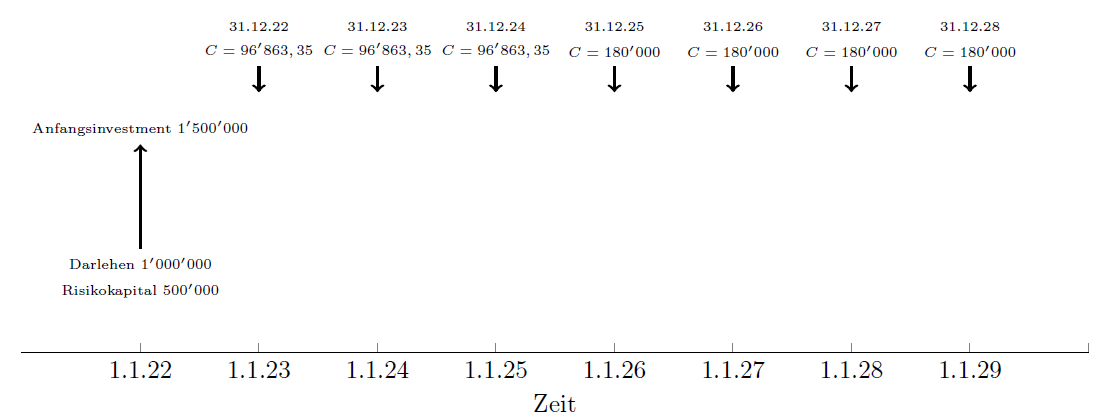
\includegraphics[scale=0.54]{pictures/zeitstrahl_1_b_filled_3}
\end{center}
\underline{(b3) 2. Berechne die Restschuld}\\
Die austehenden Schulden zum 31.12.2024 ohne das Zahlungen  getätigt werden sind:
\begin{align*}
	RS_{\mathrm{31.12.2024}}
	=
	RS_{\mathrm{1.1.2022}}
	(1 + 2 \%)^3
	= 
	1 061 208 \ \textrm{(Schweizer Franken)}.
\end{align*} 
Am 31.12.2024 beträgt der Endwert der konstanten nachschüssigen Zahlung $C_1 = 96 863.35$ Schweizer Franken beginnend am 1.1.2022:
\begin{align*}
	96863.35 \cdot
	\frac{(1+ 2 \%)^3 - 1}{2 \%}
	\approx 
	296 440.60 \ \textrm{(Schweizer Franken)}.
\end{align*}
Für die Interpretationen $C_2 $ bzw. $C_3$ ergeben sich 
$235 232.6$ bzw. $259 715.8$ Schweizer Franken
Die Restschuld am 1.1.2025 (genau nach der letzten Zahlung am 31.12.2024) ist gegeben durch:
\begin{align*}
	1 061 208
	-
	296 449.60
	=
	764 767.40 \ \textrm{(Schweizer Franken)}.
\end{align*}
Für die Interpretationen $C_2$ bzw. $C_3$ ergibt sich eine Restschuld von $825975.40$ bzw. $801492.20$ Schweizer Franken.

\newpage
\subsection*{\aufgabe{c}{10}}
Information spielt in der Entscheidungsfindung eine wesentliche Rolle. Allerdings
sehen sich Unternehmen, wie wir erst kürzlich beobachten konnten, einem Zielkonflikt
ausgesetzt. Einerseits ermöglicht das Sammeln möglichst genauer privater Informationen eine verbesserte, massgeschneiderte Lösung für ihre Kunden (die zu einem höheren Preis verkauft werden kann), andererseits erhöht es den potentiellen Schaden, den sie ihren Kunden durch Datenschutzverletzungen (und sich selbst durch mögliche juristische Folgen) zufügen könnten.\\
\\
Sei $I \geq 0 $ die Menge an Informationen, die ein Unternehmen sammelt, und $b(I)$ der Nutzen für den Kunden hinsichtlich der angebotenen Dienstleistung oder des angebotenen Produktes. Wir nehmen an, dass:
\begin{align*}
	b(I)
	= 
	\begin{cases}
		0 &\quad \textrm{für } 0 \leq I  < I_0\\
		s \left( 1 - \frac{I_0}{I} \right) & \quad \textrm{für } I \geq I_0
	\end{cases}.
\end{align*}
Demnach ist $I_0 > 0 $ die Mindestmenge an Information, die benötigt wird, um einen Nutzen für den Kunden zu generieren, und der Nutzen ist durch $s > 0 $ beschränkt, d.h., der Nutzen wird nie grösser als $s$, egal wie viel Information gesammelt wird. Im Gegensatz dazu soll der erwartete Schaden durch eine Datenschutzverletzung durch
\begin{align*}
	d(I) = \frac{1}{2} \ q \ s  \ I^2
\end{align*}
gegeben sein, wobei $q \in (0,1)$ die Wahrscheinlichkeit einer solchen Verletzung darstellt.
Zudem nehmen wir an, dass $q \  I_0^2 < \frac{8}{27}$ gilt. Für einen potentiellen Kunden ist die relevante Grösse der Trade-off $v(I)$ zwischen dem Nutzen $b(I)$ und dem möglichen Schaden $d(I)$, d.h., $v(I) = b(I) - d(I)$.\\
\\
Für welche Menge $I^\star \geq 0$ an Informationen erzielt der Kunde den bestmögliche Trade-off, d.h. den grössten Wert für $v$?
Bestimmen Sie die Antwort in Abhängigkeit der Parameter $s, I_0, q$.
Weisen Sie nach, dass $I^\star$ tatsächlich ein Maximum von $v$ ist.\\
\\
\textit{Hinweis:} Die Bedingung $q I_0^2 < \frac{8}{27}$ stellt sicher, dass $I^\star > I_0 $ gilt.\\
\\
\textbf{Lösung:}
\begin{mdframed}
\underline{\textbf{Vorgehensweise:}}
\begin{enumerate}
\item Formuliere das Optimierungsproblem.
\item Finde das Maximum $I^\star$.
\end{enumerate}
\end{mdframed}

\underline{1. Formuliere das Optimierungsproblem}\\
Das Ziel ist es den Trade-off $v(I) = b(I) - d(I)$ zwischen dem erwartetem Nutzen und dem erwarteten Schaden zu Maximieren. Hierbei ist $I$ die Informationsmenge.\\
\\
Mit dem Hinweis erhalten wir, dass mit der Bedingung $q I_0^2  < \frac{8}{27}$ auch $I^\star > I_0$ gilt, d.h. das Maximum von $v$ ist größer als $I_0$. Deswegen müssen wir nur den Fall $I > I_0$ betrachten.\\
\\
\underline{2. Finde das Maximum $I^\star$}\\
Wir schreiben zunächst $v$ für $I > I_0$ explizit auf
\begin{align*}
	v(I)
	=
	b(I) - d(I) 
	=
	s \left(1 - \frac{I_0}{I}\right)
	- \frac{1}{2} q s I_0^2
	=
	s - s \frac{I_0}{I} - \frac{1}{2} q s I_0^2
\end{align*}
und bestimmen die ersten zwei Ableitungen:
\begin{align*}
	v^\prime(I) &= s \frac{I_0}{I^2} - q s I\\
	v^{\prime \prime}(I) &= -2s \frac{I_0}{I^3} - qs
	= - \frac{2s I_0}{I^3} - qs. 
\end{align*}
Wir prüfen nun die notwendige Bedingung für einen lokalen Extrempunkt:
\begin{align*}
	v^\prime(I) = 0 
	&\ \Leftrightarrow \
	s \frac{I_0}{I^2} - q s I = 0
	\ \Leftrightarrow \
	s \frac{I_0}{I^2} = qs I 
	\ \Leftrightarrow \
	s I_0 = qs I^3
	\ \Leftrightarrow \ 
	 \frac{I_0}{q} =  I^3 \\
	 &\ \Leftrightarrow \
	   I^\star = I  = \sqrt[3]{\frac{I_0}{q}} = \left( \frac{I_0}{q}\right)^{\frac{1}{3}}.
\end{align*}
Damit haben wir mit $I^\star = \left( \frac{I_0}{q}\right)^{\frac{1}{3}}$ einen Kandidaten für ein lokales Maximum gefunden.\\
\\
Wegen  $I_0, s , q > 0$ gilt, erhalten wir für die zweite Ableitung
\begin{align*}
	v^{\prime \prime}(I)
	= -\underbrace{ \frac{2s I_0}{I^3}}_{>0} - \underbrace{qs}_{>0} < 0.
\end{align*}
für alle $I \in (I_0, \infty)$. Damit ist $v$ auf $(I_0, \infty)$ streng konkav.
Insbesondere liegt an $I^\star $ ein lokales Maximum vor, welches wegen der Konkavität auch global ist.\\
\\
Zum Abschluss noch ein paar Zusatzinformationen. Für die Bedingung des Hinweises gilt:
\begin{align*}
	q I_0^2 < \frac{8}{27}
	\ \Leftrightarrow \
	\frac{1}{q} > \frac{27 }{8} I_0^2,
\end{align*}
Hiermit ist also wirklich garantiert, dass
\begin{align*}
	I^\star 
	= 
	\left(\frac{I_0}{q}\right)^\frac{1}{3}
	>
	\left(\frac{27}{8} I_0^3\right)^\frac{1}{3}
	=
	\left(\frac{3^3}{2^3} I_0^3\right)^\frac{1}{3}
	= \frac{3}{2} I_0 > I_0
\end{align*}
gilt. Des weiteren erhalten wir:
\begin{align*}
	v(I^\star )
	&=
	s 
	\left(
		1 
		- 
		I_0 \left(\frac{I_0}{q}\right)^{-\frac{1}{3}}
		-
		\frac{1}{2} q \left(\frac{I_0}{q}\right)^{\frac{2}{3}}
	\right)\\
	&=
	s 
	\left(
	1 
	- 
	I_0^{\frac{2}{3}} q^{\frac{1}{3}}
	-
	\frac{1}{2} q^{\frac{1}{3}} I_0^\frac{2}{3}
	\right)\\
	&=
	s 
	\left(
	1 
	- 
	\frac{3}{2}
	I_0^{\frac{2}{3}} q^{\frac{1}{3}}
	\right)\\
	&> 
	s 
	\left(
	1 
	- 
	\frac{3}{2} \left(\frac{8}{27}\right)^\frac{1}{3}
	\right)
	=
	s 
	\left(
	1 
	- 
	\frac{3}{2} \cdot \frac{2}{3}
	\right)
	= 0.
\end{align*}
Somit wird durch Sammeln der optimalen Informationsmenge $I^\star$ wirklich ein echt positiver Nutzen für den Kunden erzielt.

